\chapter{Software Design}

\section{Introduction}
This chapter presents the software design of the Quantum Virtual Machine (QVM) system. The design follows object-oriented principles and emphasizes modularity, maintainability, and extensibility. The chapter documents the architectural decisions, design patterns, and structural organization that enable the QVM to achieve its goal of hardware-agnostic quantum circuit execution. The design is presented through multiple perspectives using UML diagrams, including architectural views, behavioral models, and data flow representations.

\section{Design Methodology}
The QVM system was designed using \textbf{Object-Oriented Design (OOD)} methodology with emphasis on the following principles:

\textbf{Separation of Concerns:} The system is divided into distinct modules (Parser, IR, Transpiler, Simulator, Visualizer) with well-defined responsibilities. Each module encapsulates a specific aspect of the quantum compilation and execution pipeline.

\textbf{Pipeline Architecture:} The design follows a linear pipeline pattern where data flows through sequential stages of transformation: Input → Parsing → IR → Transpilation → Simulation → Output. This architecture mirrors the natural workflow of quantum program execution.

\textbf{Strategy Pattern:} The transpiler module implements the Strategy pattern, allowing runtime selection between different routing algorithms (Greedy BFS, SABRE) without modifying client code.

\textbf{Abstraction and Interfaces:} The QuantumCircuit IR serves as an abstraction layer that decouples high-level circuit definitions from low-level execution details, enabling hardware independence.

\textbf{Modularity and Extensibility:} Each component is designed as an independent module with minimal coupling, allowing new parsers, simulators, or transpilation strategies to be added without affecting existing code.

\section{System Overview}
The QVM system architecture is organized as a layered pipeline with clear boundaries between components. Figure \ref{fig:context} shows the system context, illustrating how the QVM interacts with external actors (developers, students, administrators) and external systems (file system, web browsers, IBM Quantum platform). The system accepts quantum programs through three interfaces (CLI, Web API, Web GUI) and produces results in multiple formats (statevector, probabilities, visualizations, OpenQASM export).

\begin{sidewaysfigure}
\centering
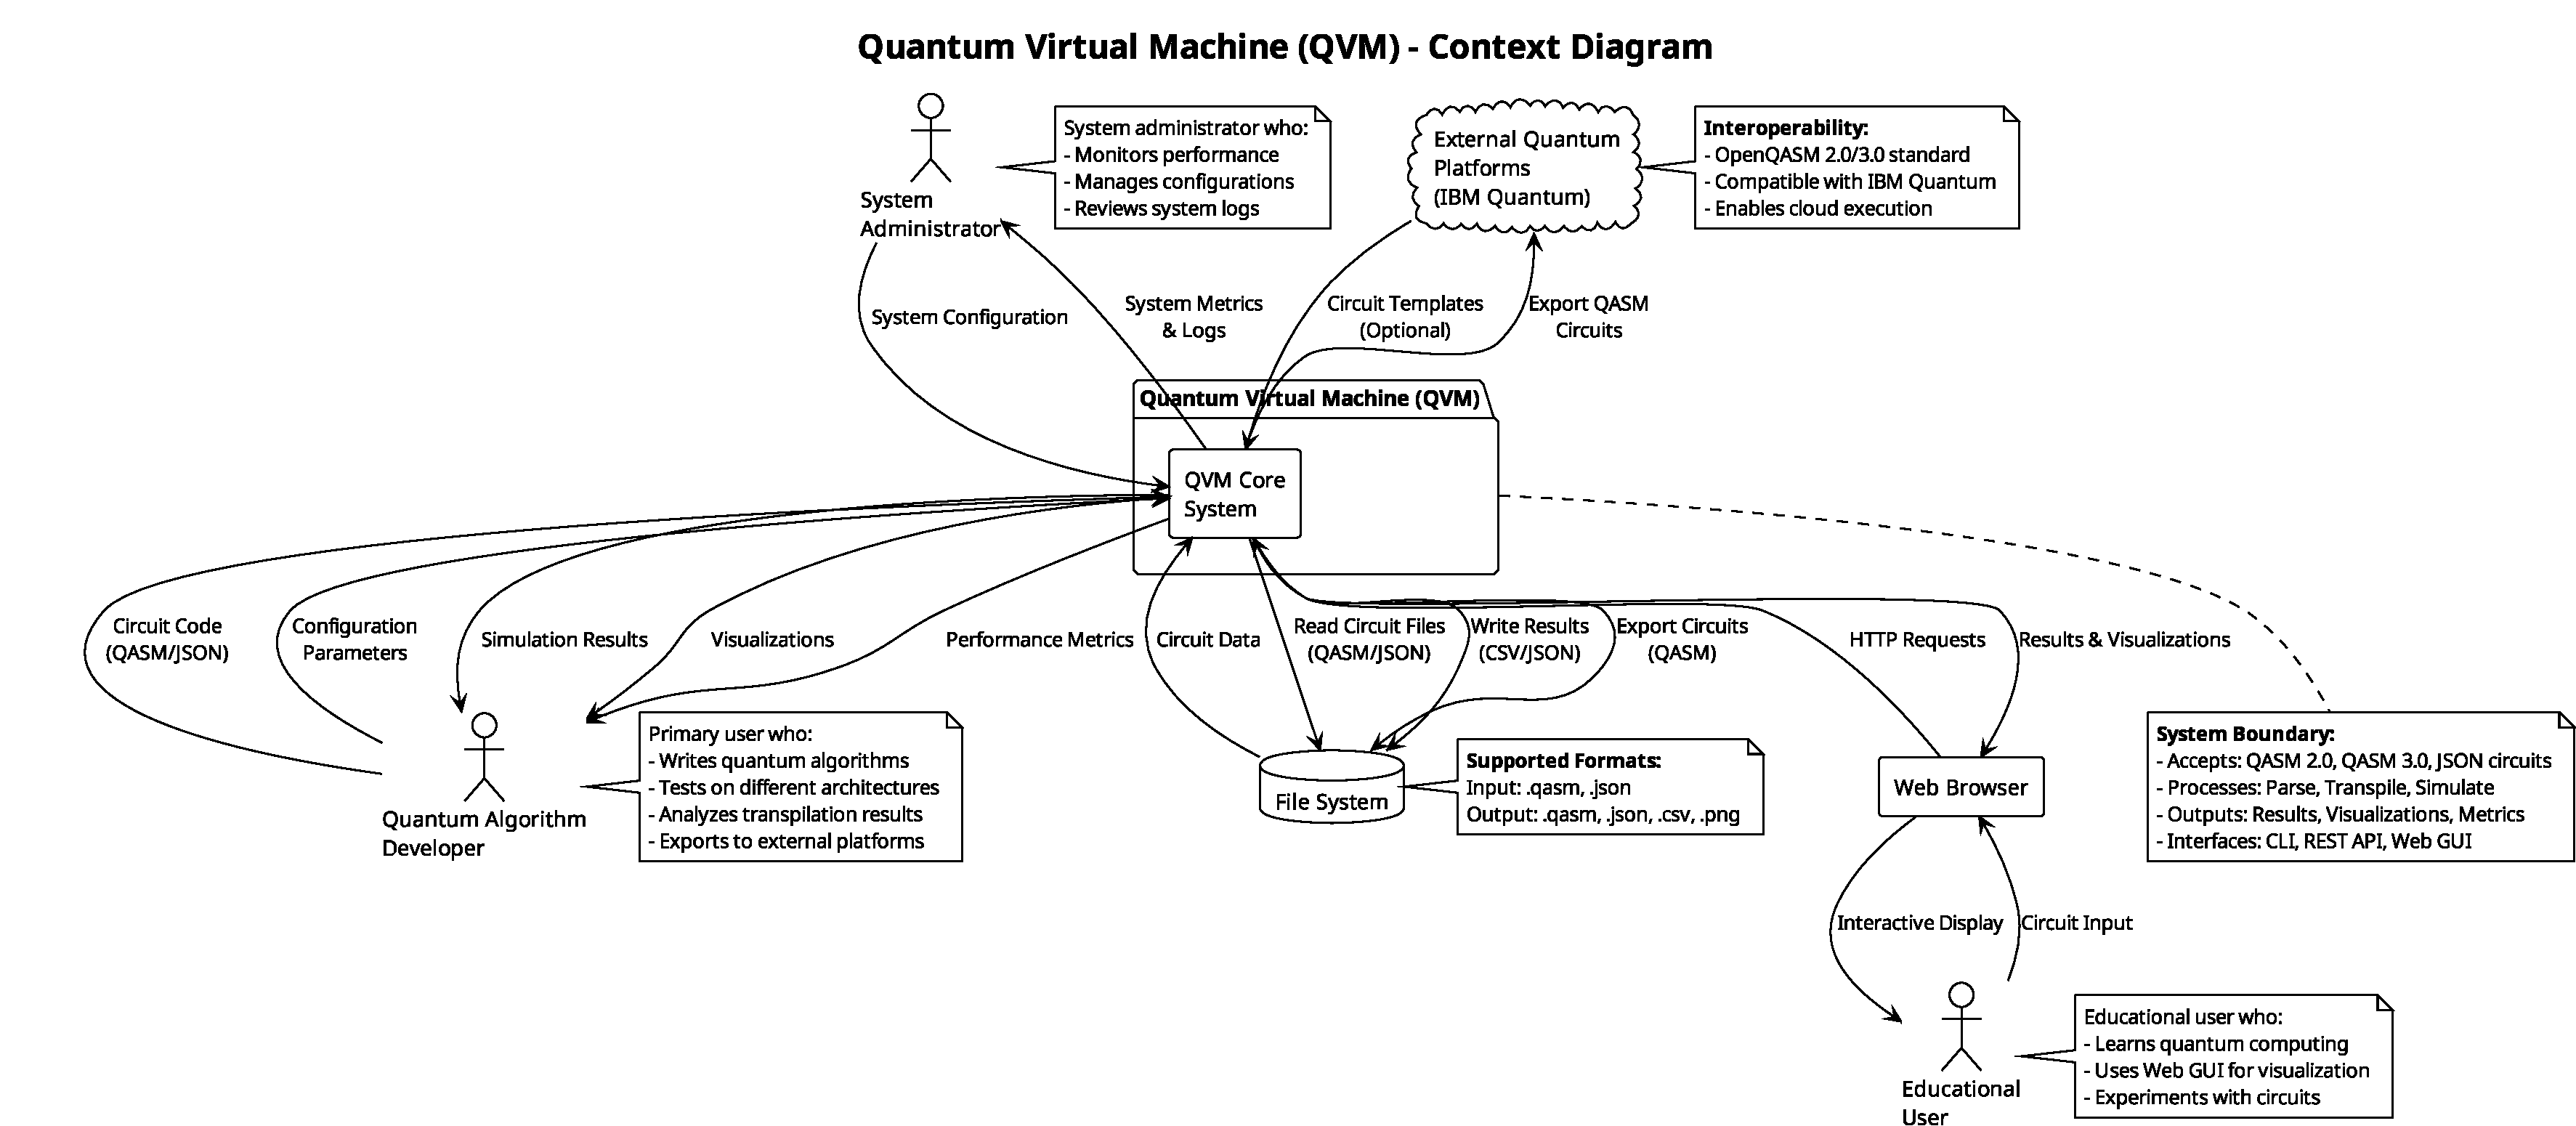
\includegraphics[width=0.95\linewidth,height=0.95\textheight,keepaspectratio]{../uml/QVM_Context_Diagram.pdf}
\caption{System Context Diagram}
\label{fig:context}
\end{sidewaysfigure}

The context diagram establishes the system boundary and identifies all external entities that interact with the QVM. Users provide quantum circuits as input and receive execution results as output. The system reads circuit files from the file system and can export results back to files. The web-based interfaces communicate with browsers via HTTP, and the OpenQASM export capability enables integration with external quantum platforms like IBM Quantum.

\section{Architectural Design}
The QVM follows a \textbf{7-layer pipeline architecture} as shown in Figure \ref{fig:architecture}. Each layer represents a distinct phase in the quantum program lifecycle:

\begin{figure}[H]
\centering

\includegraphics[page=1,width=0.95\textwidth]{../uml/split/QVM_Architecture_Diagram.pdf}
\caption{System Architecture Diagram (Part 1 of 3)}
\end{figure}

\begin{figure}[H]
\centering

\includegraphics[page=2,width=0.95\textwidth]{../uml/split/QVM_Architecture_Diagram.pdf}
\caption{System Architecture Diagram (Part 2 of 3)}
\end{figure}

\begin{figure}[H]
\centering

\includegraphics[page=3,width=0.95\textwidth]{../uml/split/QVM_Architecture_Diagram.pdf}
\caption{System Architecture Diagram (Part 3 of 3)}
\label{fig:architecture}
\end{figure}

\textbf{Layer 1 - Input Layer:} Accepts quantum programs in three formats (OpenQASM 3.0, OpenQASM 2.0, JSON) through three interfaces (CLI, Web API, Web GUI). This layer provides flexibility in how users interact with the system.

\textbf{Layer 2 - Parser Layer:} Transforms textual circuit descriptions into structured Abstract Syntax Trees (AST). Uses Lark parser generator for OpenQASM 3.0 with formal grammar definition. Validates syntax and semantics before proceeding.

\textbf{Layer 3 - Intermediate Representation (IR):} Converts AST into a hardware-agnostic QuantumCircuit object. This layer decouples the input format from the execution backend, enabling the "Write Once, Run Anywhere" philosophy.

\textbf{Layer 4 - Decomposer:} Breaks down complex gates (Toffoli, controlled gates) into native gate sets supported by target architectures. Maps high-level operations to primitive gates (H, X, Y, Z, CX).

\textbf{Layer 5 - Transpiler:} Maps logical qubits to physical qubits according to hardware topology constraints. Implements two routing strategies (Greedy BFS, SABRE) and inserts SWAP gates to satisfy connectivity requirements.

\textbf{Layer 6 - Simulator:} Executes the transpiled circuit using either exact statevector simulation (up to 12 qubits) or efficient Matrix Product State (MPS) simulation (20+ qubits for low-entanglement circuits). Maintains classical memory for hybrid quantum-classical computation.

\textbf{Layer 7 - Output Layer:} Produces results in multiple formats: final statevector, measurement probabilities, circuit visualizations (matplotlib), and OpenQASM export for external tools.

This layered architecture ensures that each component has a single, well-defined responsibility and can be tested, modified, or replaced independently.

\section{Activity Diagrams}
Activity diagrams model the dynamic behavior of the system by showing the flow of control through various processes. The QVM system has three primary workflows:

\subsection{Circuit Execution Flow}
Figure \ref{fig:activity_execution} shows the complete workflow from loading a circuit file to displaying results. The process includes error handling for invalid files and syntax errors, backend selection (Statevector vs MPS), optional transpilation, and result visualization.

\begin{figure}[H]
\centering

\includegraphics[page=1,width=0.95\textwidth]{../uml/split/Activity_Circuit_Execution.pdf}
\caption{Activity Diagram - Circuit Execution Flow (Part 1 of 2)}
\end{figure}

\begin{figure}[H]
\centering

\includegraphics[page=2,width=0.95\textwidth]{../uml/split/Activity_Circuit_Execution.pdf}
\caption{Activity Diagram - Circuit Execution Flow (Part 2 of 2)}
\label{fig:activity_execution}
\end{figure}

The execution flow begins with the user providing a circuit file. The system validates the file existence and format, then invokes the appropriate parser. If parsing succeeds, the user can optionally request transpilation for a specific architecture. The system then selects the appropriate simulator based on circuit size and user preference. After simulation, results are displayed and optionally saved to files.

\subsection{Transpilation Process}
Figure \ref{fig:activity_transpile} details the transpilation workflow, showing how logical circuits are mapped to physical hardware topologies. The process includes gate decomposition, qubit routing (with choice between Greedy and SABRE algorithms), SWAP insertion, and optional mapping restoration.

\begin{figure}[H]
\centering

\includegraphics[page=1,width=0.95\textwidth]{../uml/split/Activity_Transpilation.pdf}
\caption{Activity Diagram - Transpilation Process (Part 1 of 3)}
\end{figure}

\begin{figure}[H]
\centering

\includegraphics[page=2,width=0.95\textwidth]{../uml/split/Activity_Transpilation.pdf}
\caption{Activity Diagram - Transpilation Process (Part 2 of 3)}
\end{figure}

\begin{figure}[H]
\centering

\includegraphics[page=3,width=0.95\textwidth]{../uml/split/Activity_Transpilation.pdf}
\caption{Activity Diagram - Transpilation Process (Part 3 of 3)}
\label{fig:activity_transpile}
\end{figure}

The transpilation process starts by analyzing the logical circuit's connectivity requirements. Complex gates are decomposed into native gates. The routing algorithm then determines the optimal qubit mapping, inserting SWAP gates where necessary to satisfy topology constraints. If mapping restoration is enabled, additional SWAPs are inserted to return qubits to their original logical positions.

\subsection{Simulation Process}
Figure \ref{fig:activity_simulate} illustrates the simulation workflow, including state initialization, gate application, measurement with collapse, and control flow handling (labels, jumps, conditionals).

\begin{sidewaysfigure}
\centering
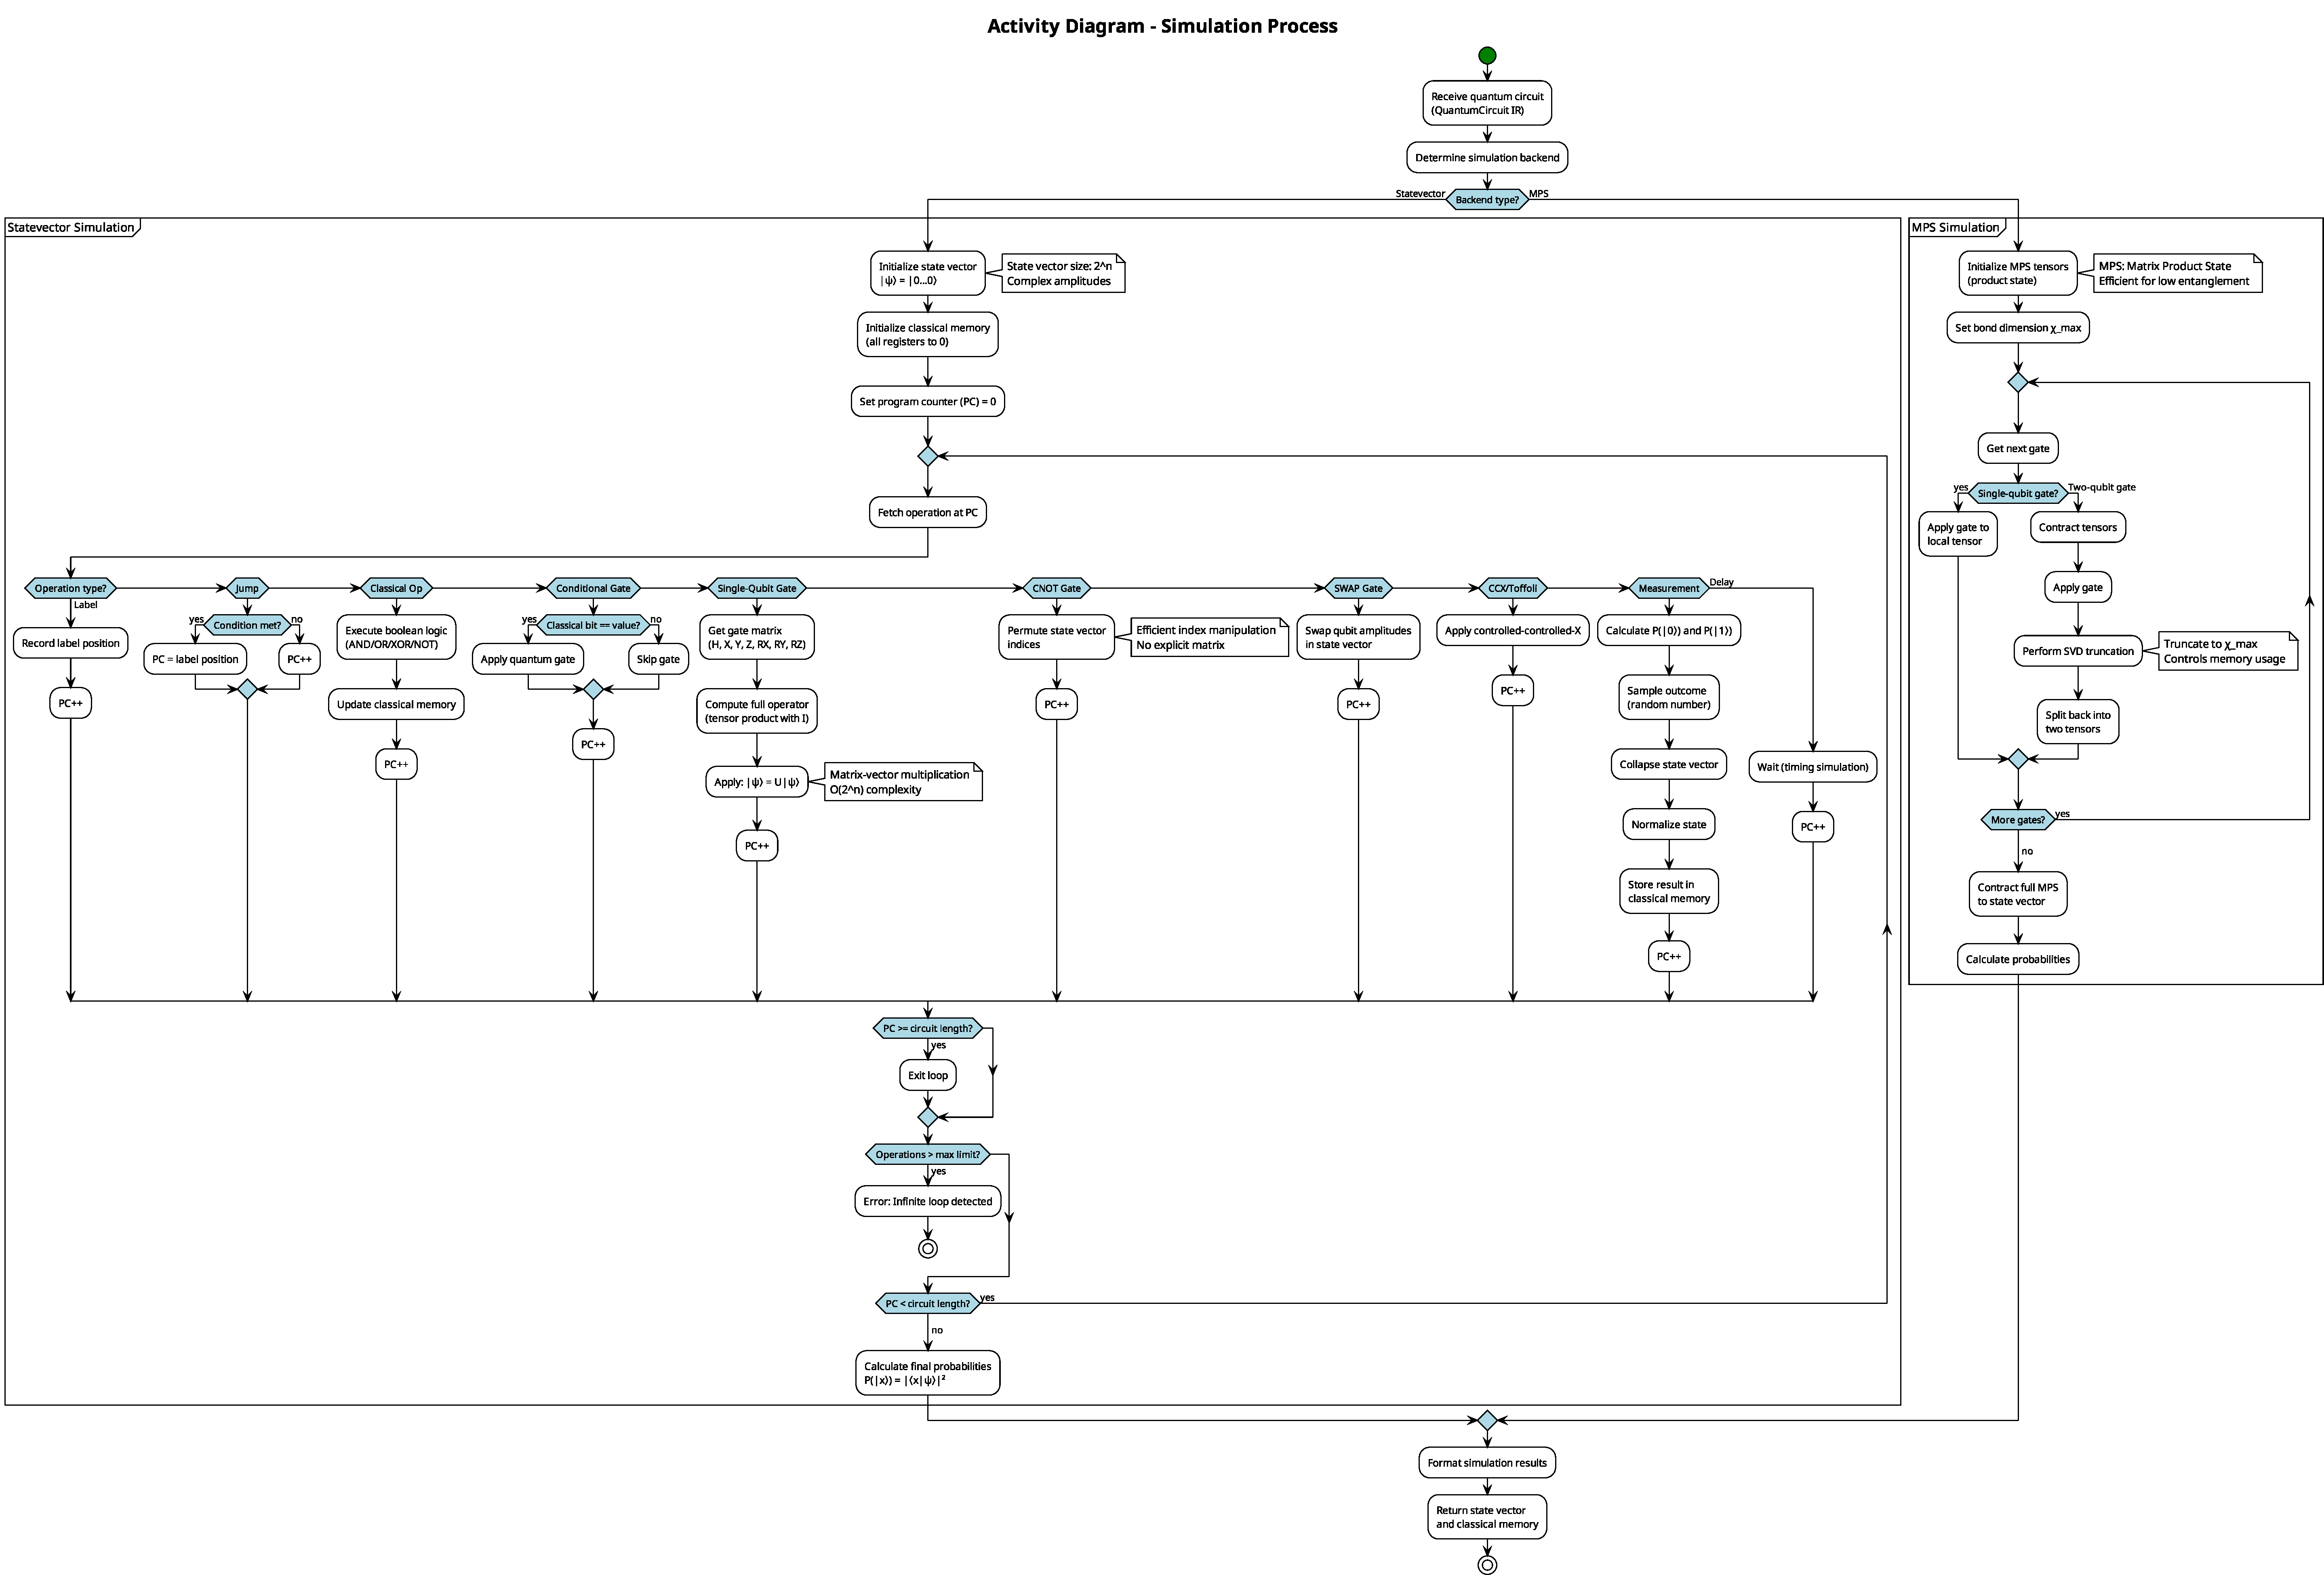
\includegraphics[width=0.95\linewidth,height=0.95\textheight,keepaspectratio]{../uml/Activity_Simulation.pdf}
\caption{Activity Diagram - Simulation Process}
\label{fig:activity_simulate}
\end{sidewaysfigure}

The simulation process initializes the quantum state to $|0\rangle^{\otimes n}$ and classical memory to zeros. It then iterates through circuit operations, applying unitary transformations for gates, performing probabilistic collapse for measurements, and updating classical memory. Control flow operations (if, while, jump) are handled by maintaining a program counter and label map. The process includes infinite loop detection to prevent runaway execution.

\section{Class Diagram}
The class diagram in Figure \ref{fig:class} shows the static structure of the QVM system, including all major classes, their attributes, methods, and relationships.

\begin{sidewaysfigure}
\centering

\includegraphics[width=0.95\linewidth,height=0.95\textheight,keepaspectratio]{../uml/QVM_Class_Diagram.pdf}
\caption{Class Diagram - System Structure}
\label{fig:class}
\end{sidewaysfigure}

\textbf{Core Classes:}

\textbf{QuantumCircuit:} The central IR class that represents a hardware-agnostic quantum circuit. Contains num\_qubits, operations list, and classical\_registers dictionary. Provides methods for adding operations, classical registers, and string representation.

\textbf{Simulator:} Implements exact statevector simulation using NumPy. Contains gate matrices (H, X, Y, Z, CX, etc.) and methods for applying gates, measurements, and control flow. The simulate() method returns the final statevector and classical memory state.

\textbf{MPSSimulator:} Implements Matrix Product State simulation for efficient handling of low-entanglement circuits. Uses tensor contractions and SVD truncation to maintain computational efficiency.

\textbf{Transpiler:} Maps logical circuits to physical architectures. Contains target\_architecture, strategy (greedy/sabre), and restore\_mapping flag. Implements BFS routing, SABRE heuristics, and SWAP insertion algorithms.

\textbf{OpenQASM3Parser:} Parses OpenQASM 3.0 files using Lark grammar. Implements two-pass parsing: first pass for declarations, second pass for operations. Handles control flow (if, for, while) and classical operations.

\textbf{QASMParser:} Parses OpenQASM 2.0 files with basic gate support. Simpler than OpenQASM3Parser but sufficient for standard quantum algorithms.

\textbf{TargetArchitecture:} Represents hardware topology with num\_qubits and connectivity list. Provides is\_connected() method to check if two qubits are adjacent.

\textbf{Decomposer:} Breaks down complex gates into native gate sets. Implements decomposition rules (e.g., Toffoli → CNOTs + single-qubit gates).

\textbf{Visualizer:} Generates circuit diagrams and probability histograms using matplotlib. Provides draw\_circuit() and plot\_probabilities() methods.

\textbf{CLI:} Command-line interface that parses arguments and orchestrates the execution pipeline. Handles file loading, transpilation options, and result display.

\textbf{APIServer:} FastAPI-based REST API server. Provides /execute endpoint that accepts JSON circuit definitions and returns JSON results.

\textbf{Relationships:}
- Simulator and MPSSimulator both depend on QuantumCircuit
- Transpiler depends on QuantumCircuit and TargetArchitecture
- Parsers create QuantumCircuit objects
- CLI and APIServer orchestrate all components

\section{Sequence Diagrams}
Sequence diagrams show the dynamic interactions between objects over time. The QVM system has three key interaction scenarios:

\subsection{CLI Execution Flow}
Figure \ref{fig:seq_cli} shows the interaction sequence when a user executes a circuit via the command-line interface.

\begin{figure}[H]
\centering

\includegraphics[page=1,width=0.95\textwidth]{../uml/split/Sequence_CLI_Execution.pdf}
\caption{Sequence Diagram - CLI Execution (Part 1 of 2)}
\end{figure}

\begin{figure}[H]
\centering

\includegraphics[page=2,width=0.95\textwidth]{../uml/split/Sequence_CLI_Execution.pdf}
\caption{Sequence Diagram - CLI Execution (Part 2 of 2)}
\label{fig:seq_cli}
\end{figure}

The sequence begins with the user invoking the CLI with a circuit file. The CLI loads the file and delegates to the Parser, which creates a QuantumCircuit IR. If transpilation is requested, the CLI invokes the Transpiler with the target architecture. The Transpiler returns a physical circuit with SWAP gates inserted. The CLI then invokes the Simulator, which executes the circuit and returns the statevector and classical memory. Finally, the CLI invokes the Visualizer to display results to the user.

\subsection{API Request Flow}
Figure \ref{fig:seq_api} illustrates the interaction when a client submits a circuit via the REST API.

\begin{figure}[H]
\centering

\includegraphics[page=1,width=0.95\textwidth]{../uml/split/Sequence_API_Request.pdf}
\caption{Sequence Diagram - API Request (Part 1 of 3)}
\end{figure}

\begin{figure}[H]
\centering

\includegraphics[page=2,width=0.95\textwidth]{../uml/split/Sequence_API_Request.pdf}
\caption{Sequence Diagram - API Request (Part 2 of 3)}
\end{figure}

\begin{figure}[H]
\centering

\includegraphics[page=3,width=0.95\textwidth]{../uml/split/Sequence_API_Request.pdf}
\caption{Sequence Diagram - API Request (Part 3 of 3)}
\label{fig:seq_api}
\end{figure}

The client sends an HTTP POST request with a JSON circuit definition. The APIServer validates the request format and extracts the circuit data. It then delegates to the Parser to create a QuantumCircuit IR. The APIServer invokes the Simulator to execute the circuit. After receiving the results, the APIServer formats them as JSON and returns an HTTP 200 response to the client. Error handling is included for invalid JSON (HTTP 400) and execution errors (HTTP 500).

\subsection{Transpilation Detail}
Figure \ref{fig:seq_transpile} shows the detailed interaction during the transpilation process.

\begin{figure}[H]
\centering

\includegraphics[page=1,width=0.95\textwidth]{../uml/split/Sequence_Transpilation_Detail.pdf}
\caption{Sequence Diagram - Transpilation Detail (Part 1 of 3)}
\end{figure}

\begin{figure}[H]
\centering

\includegraphics[page=2,width=0.95\textwidth]{../uml/split/Sequence_Transpilation_Detail.pdf}
\caption{Sequence Diagram - Transpilation Detail (Part 2 of 3)}
\end{figure}

\begin{figure}[H]
\centering

\includegraphics[page=3,width=0.95\textwidth]{../uml/split/Sequence_Transpilation_Detail.pdf}
\caption{Sequence Diagram - Transpilation Detail (Part 3 of 3)}
\label{fig:seq_transpile}
\end{figure}

The Transpiler receives a logical circuit and target architecture. It first invokes the Decomposer to break down complex gates. The Decomposer returns a circuit with only native gates. The Transpiler then analyzes connectivity requirements and selects the routing strategy (Greedy or SABRE). For each two-qubit gate that violates topology constraints, the Transpiler inserts SWAP gates to bring qubits into adjacency. The process continues until all gates satisfy connectivity requirements. If mapping restoration is enabled, additional SWAPs are inserted to restore the original logical-to-physical mapping.

\section{State Transition Diagrams}
State transition diagrams model the lifecycle of key entities in the system. Figure \ref{fig:state} shows the state transitions for a quantum circuit as it progresses through the QVM pipeline.

\begin{figure}[H]
\centering
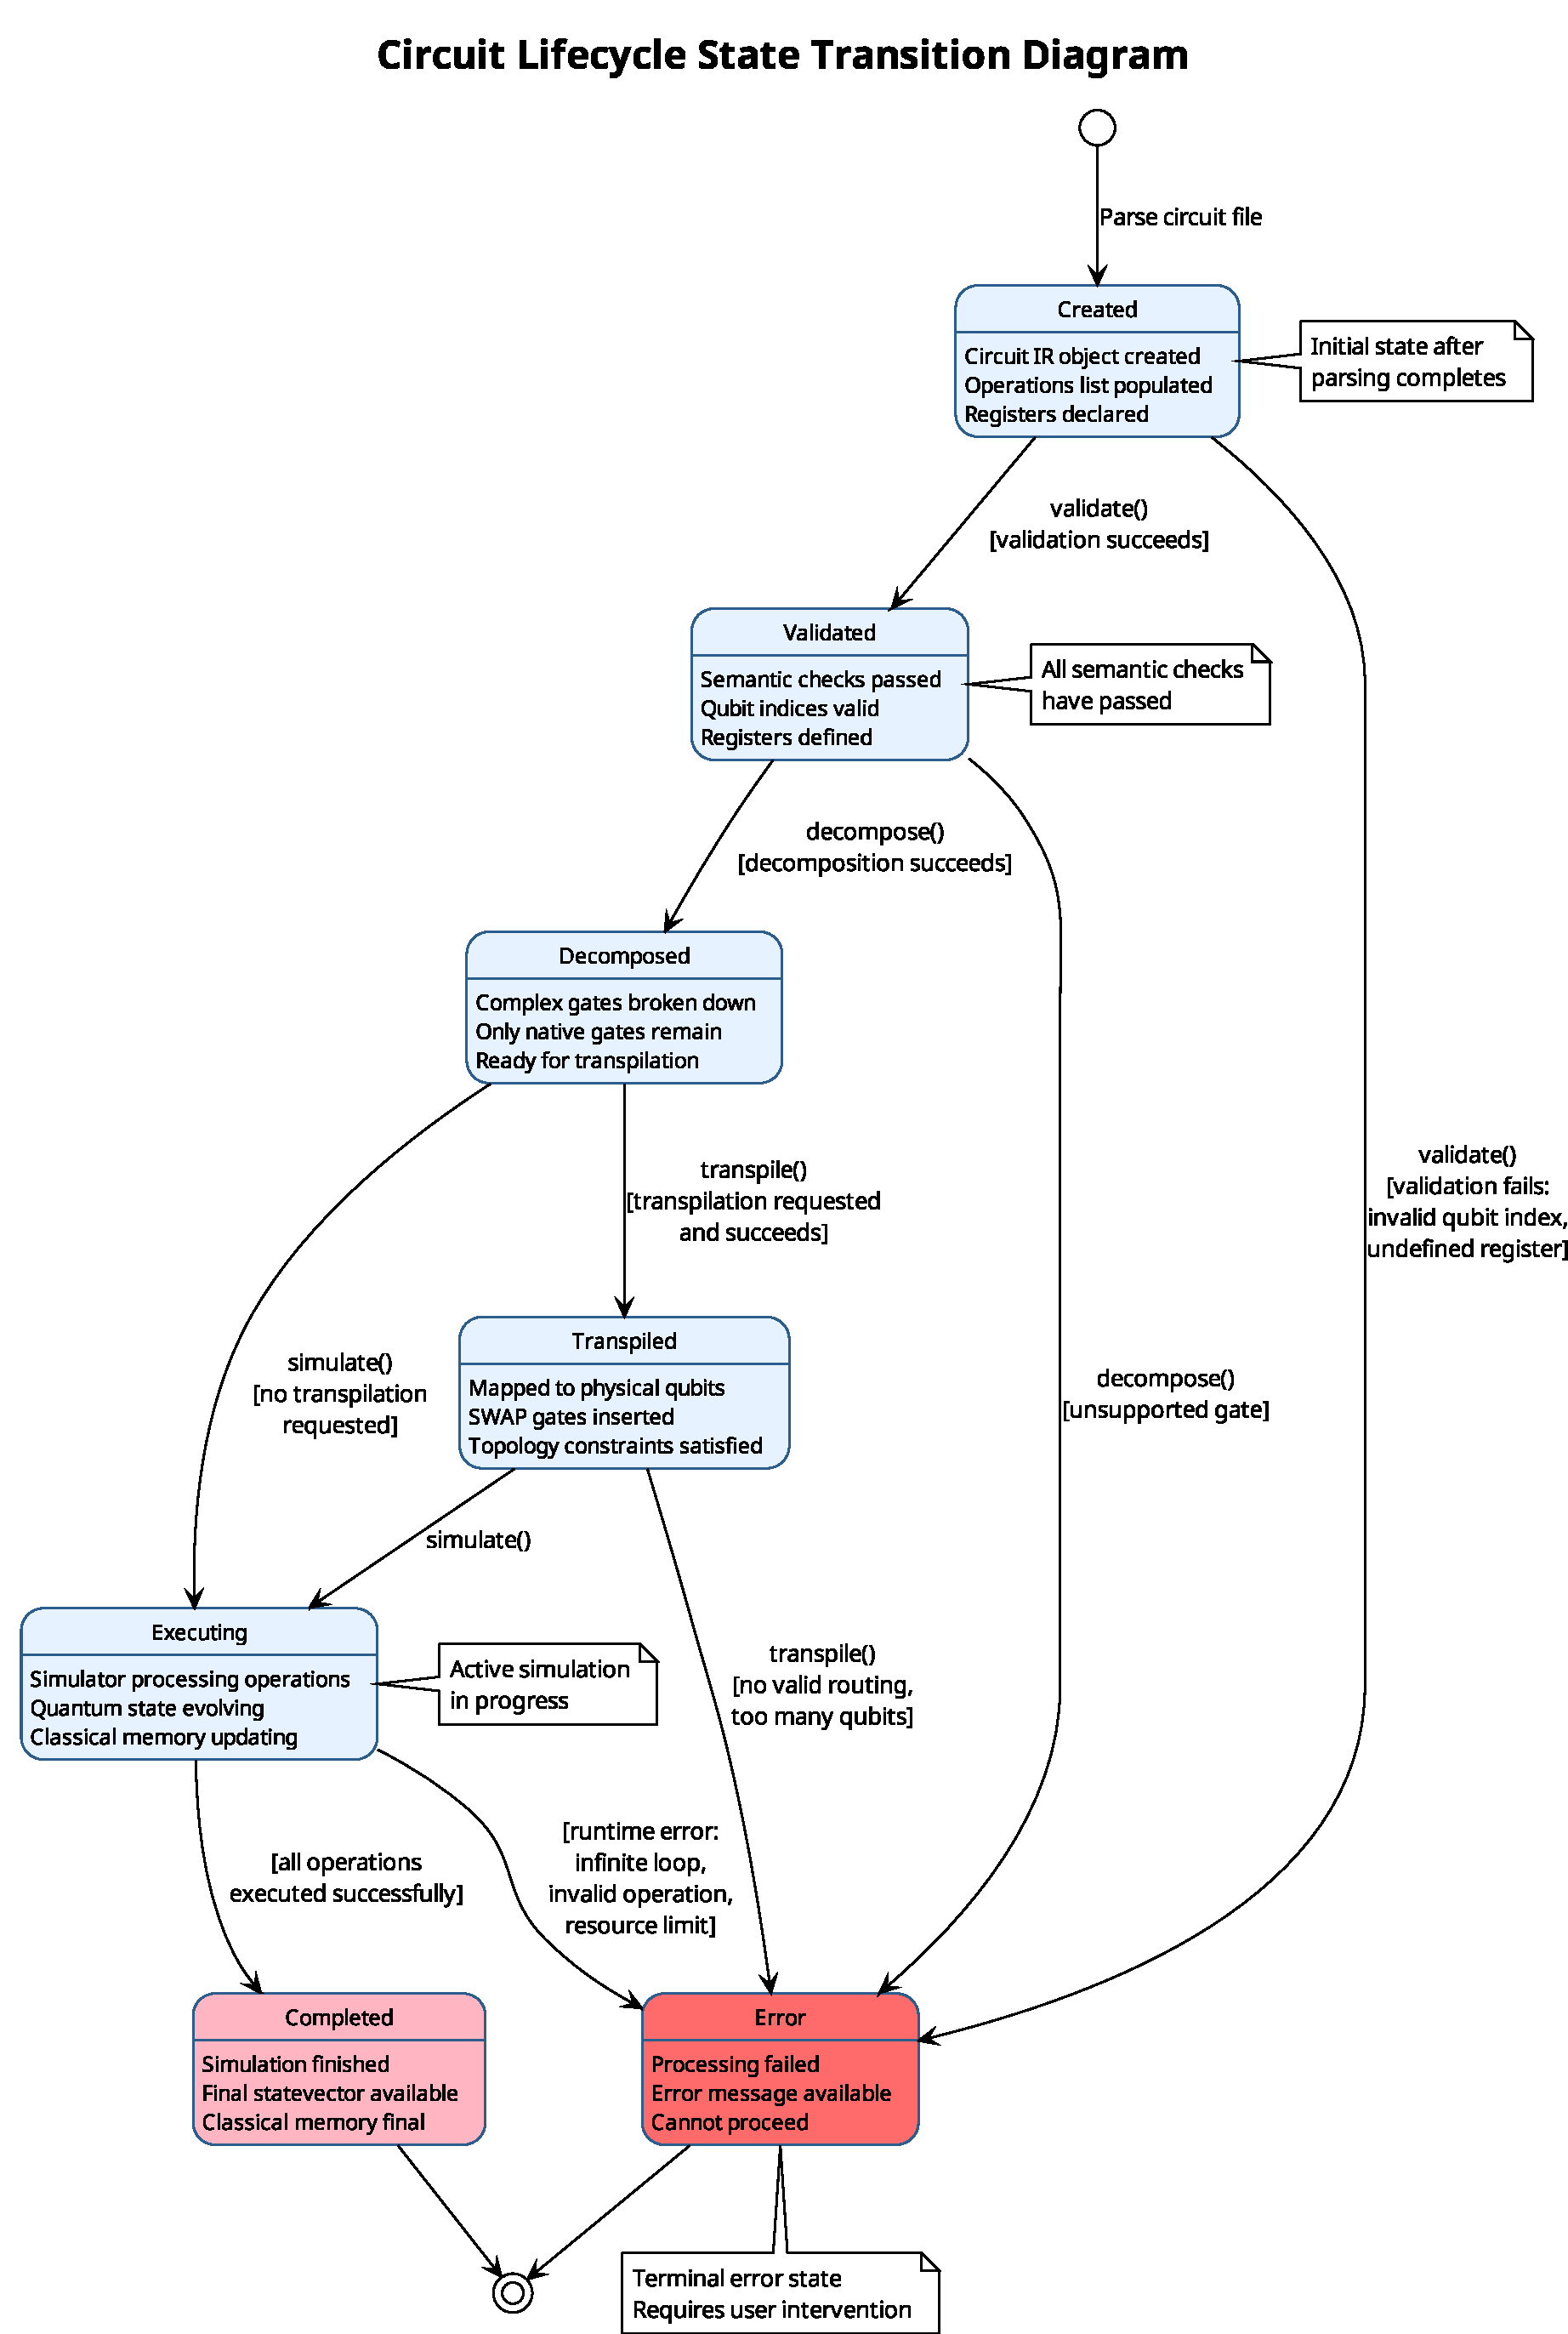
\includegraphics[width=0.85\textwidth,height=0.8\textheight,keepaspectratio]{../uml/State_Circuit_Lifecycle.pdf}
\caption{State Transition Diagram - Circuit Lifecycle}
\label{fig:state}
\end{figure}

\textbf{Circuit States:}

\textbf{Created:} Initial state after parsing. The circuit exists as a QuantumCircuit IR object but has not been validated or processed.

\textbf{Validated:} The circuit has passed semantic validation (qubit indices in range, valid gate parameters, classical registers declared).

\textbf{Decomposed:} Complex gates have been broken down into native gate sets. The circuit now contains only primitive operations.

\textbf{Transpiled:} The circuit has been mapped to a physical architecture with SWAP gates inserted. Logical qubits are mapped to physical qubits.

\textbf{Executing:} The simulator is actively processing the circuit operations. The quantum state is being evolved step-by-step.

\textbf{Completed:} Simulation has finished successfully. The final statevector and classical memory are available.

\textbf{Error:} An error occurred during any stage (parsing, validation, transpilation, or execution). The circuit cannot proceed further.

\textbf{State Transitions:}
- Created → Validated: Semantic validation succeeds
- Created → Error: Validation fails (invalid qubit index, undefined register)
- Validated → Decomposed: Gate decomposition succeeds
- Decomposed → Transpiled: Transpilation succeeds (or skipped if not requested)
- Transpiled → Executing: Simulation begins
- Executing → Completed: All operations executed successfully
- Executing → Error: Runtime error (infinite loop, invalid operation)

\section{Data Flow Diagrams}

\subsection{Level 1 DFD - System Level}
Figure \ref{fig:dfd1} shows the high-level data flows between the QVM system and external entities.

\begin{sidewaysfigure}
\centering
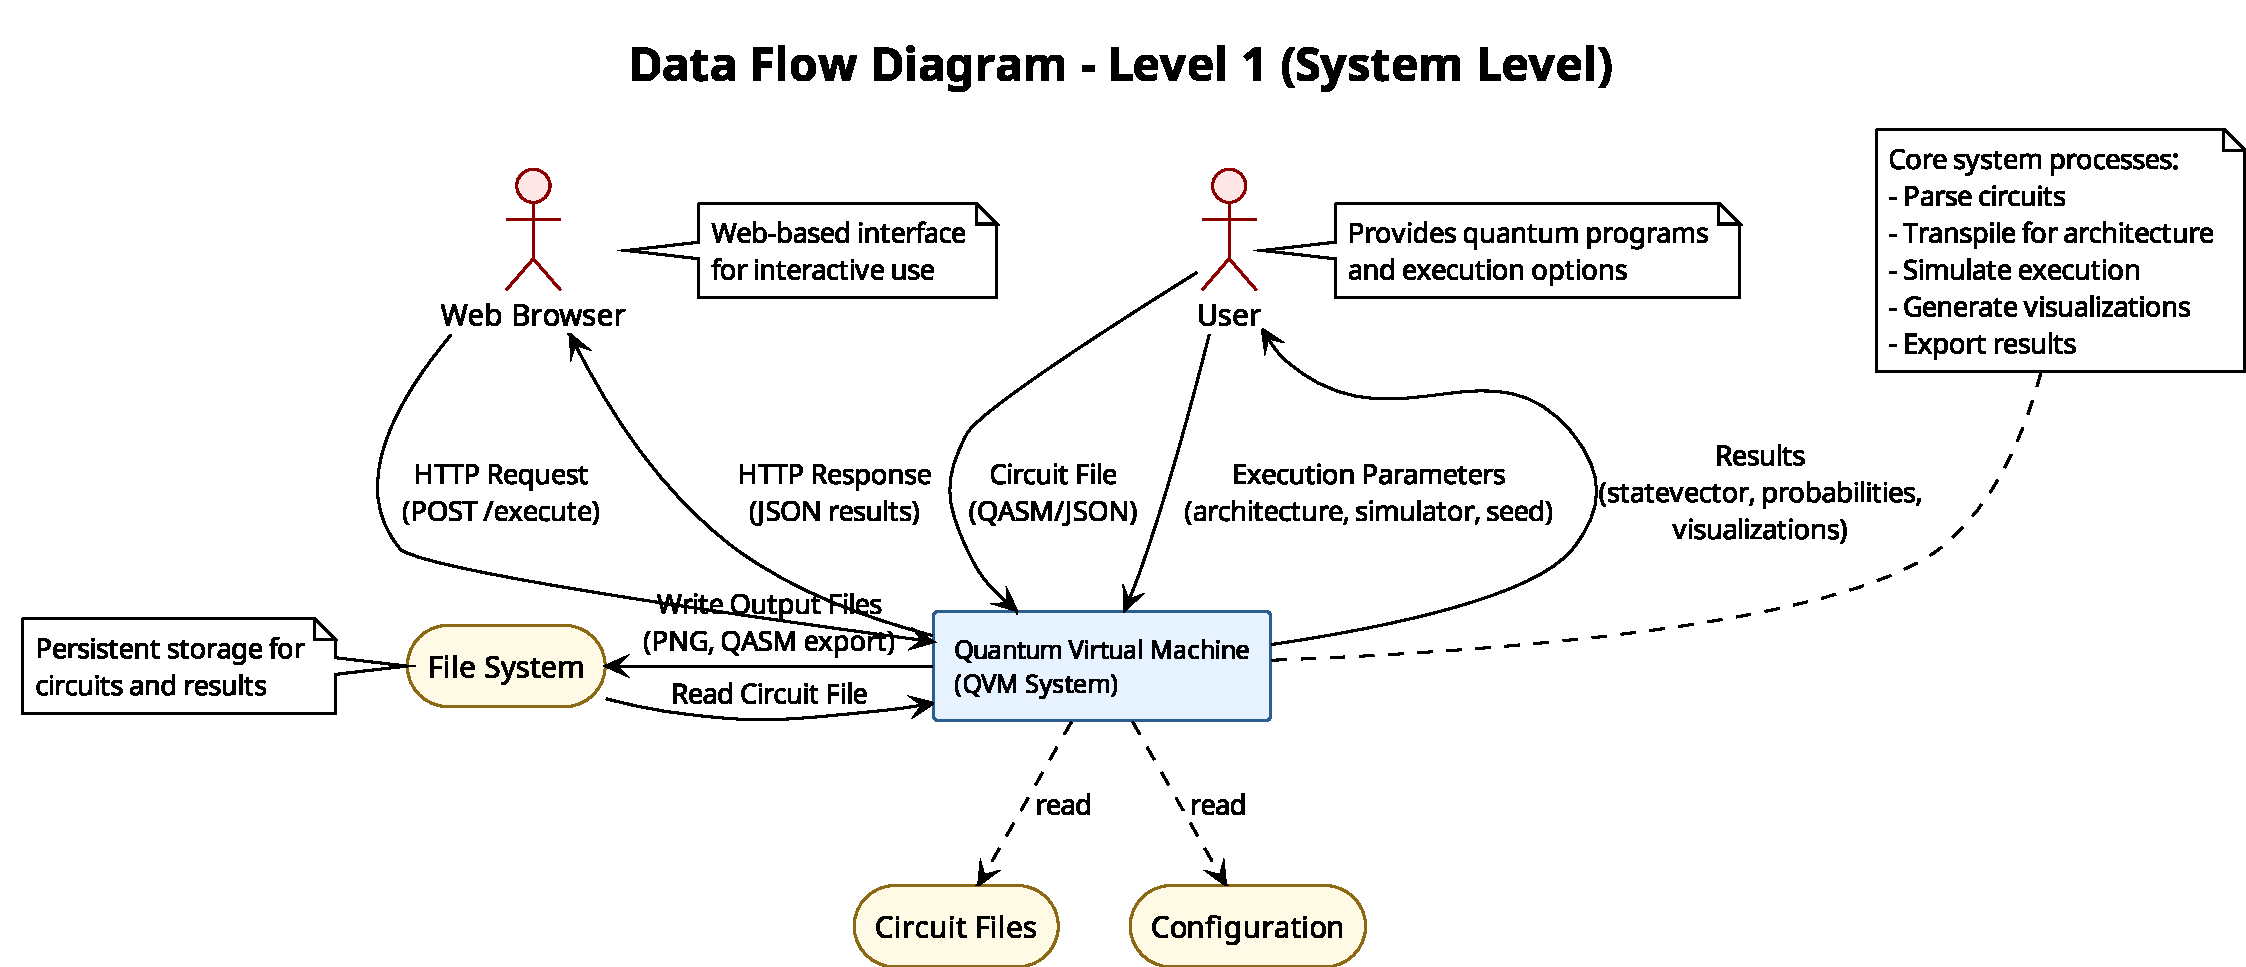
\includegraphics[width=0.95\linewidth,height=0.95\textheight,keepaspectratio]{../uml/DFD_Level1.pdf}
\caption{Data Flow Diagram - Level 1 (System Level)}
\label{fig:dfd1}
\end{sidewaysfigure}

\textbf{External Entities:}
- User: Provides circuit files and execution parameters
- File System: Stores circuit files and output results
- Web Browser: Displays web GUI and receives results

\textbf{Data Flows:}
- Circuit File → QVM System: User provides quantum program
- Execution Parameters → QVM System: User specifies options (architecture, simulator, seed)
- Results → User: System returns statevector, probabilities, visualizations
- Circuit File ← File System: System reads input files
- Output Files → File System: System writes visualizations and exports
- HTTP Request → QVM System: Browser sends circuit via API
- HTTP Response → Web Browser: System returns JSON results

\textbf{Data Stores:}
- Circuit Files: Persistent storage of quantum programs
- Configuration: System settings and architecture definitions

\subsection{Level 2 DFD - Module Level}
Figure \ref{fig:dfd2} shows the detailed data flows between internal modules.

\begin{sidewaysfigure}
\centering
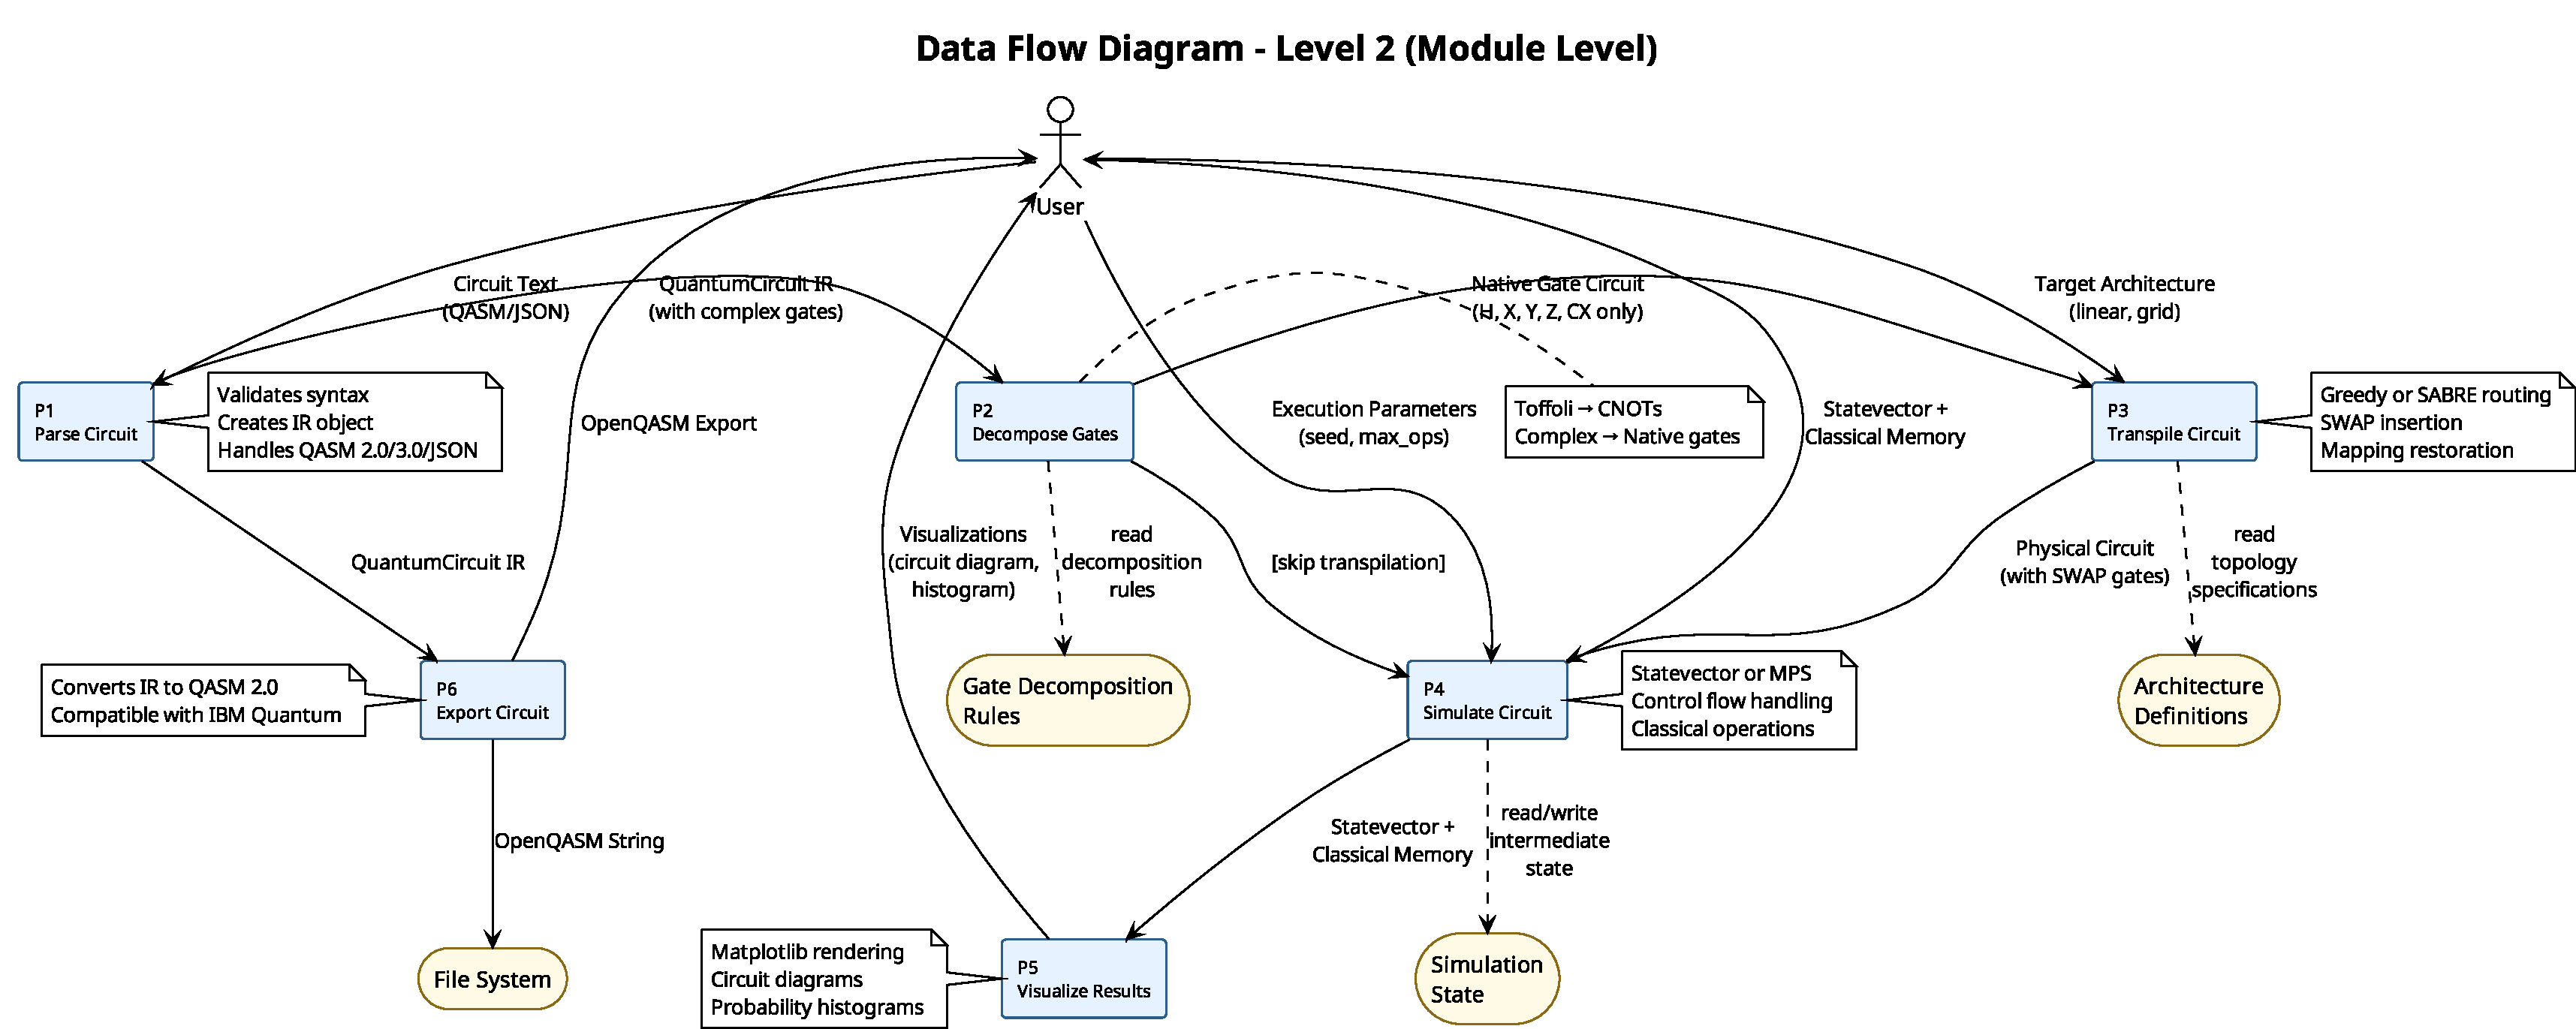
\includegraphics[width=0.95\linewidth,height=0.95\textheight,keepaspectratio]{../uml/DFD_Level2.pdf}
\caption{Data Flow Diagram - Level 2 (Module Level)}
\label{fig:dfd2}
\end{sidewaysfigure}

\textbf{Processes:}

\textbf{P1 - Parse Circuit:} Accepts circuit text and produces QuantumCircuit IR. Validates syntax and semantics.

\textbf{P2 - Decompose Gates:} Accepts QuantumCircuit with complex gates and produces QuantumCircuit with native gates only.

\textbf{P3 - Transpile Circuit:} Accepts logical QuantumCircuit and target architecture, produces physical QuantumCircuit with SWAP gates.

\textbf{P4 - Simulate Circuit:} Accepts QuantumCircuit and execution parameters, produces statevector and classical memory.

\textbf{P5 - Visualize Results:} Accepts statevector and circuit, produces diagrams and histograms.

\textbf{P6 - Export Circuit:} Accepts QuantumCircuit, produces OpenQASM string.

\textbf{Data Flows:}
- Circuit Text → P1: Raw input from file or API
- QuantumCircuit IR → P2: Parsed circuit with all gates
- Native Gate Circuit → P3: Circuit with only primitive gates
- Physical Circuit → P4: Transpiled circuit ready for execution
- Statevector + Classical Memory → P5: Simulation results
- QuantumCircuit IR → P6: Circuit to be exported
- OpenQASM String → User: Exported circuit for external tools

\textbf{Data Stores:}
- Architecture Definitions: Topology specifications (linear, grid)
- Gate Decomposition Rules: Mapping from complex gates to native gates
- Simulation State: Intermediate quantum state during execution

\section{Entity-Relationship Diagram}
The QVM system does not use a traditional relational database. Instead, it uses a \textbf{file-based data model} where quantum circuits are stored as text files (OpenQASM, JSON) and results are stored as output files (PNG images, QASM exports).

\textbf{Rationale for File-Based Approach:}
\begin{itemize}
\item \textbf{Simplicity:} Quantum circuits are naturally represented as text files, making them human-readable and version-controllable.
\item \textbf{Portability:} File-based storage allows easy sharing of circuits between users and systems without database dependencies.
\item \textbf{Stateless Execution:} Each circuit execution is independent, requiring no persistent state between runs.
\item \textbf{Educational Focus:} File-based approach is easier for students to understand and debug compared to database abstractions.
\end{itemize}

\textbf{File Structure:}
\begin{itemize}
\item \textbf{Input Files:} .qasm (OpenQASM 2.0/3.0), .json (JSON gate lists)
\item \textbf{Output Files:} .png (visualizations), .qasm (exports), .txt (results)
\item \textbf{Configuration Files:} .json (architecture definitions)
\end{itemize}

If the system were to be extended with a database for storing execution history or user accounts, a simple schema would include:
\begin{itemize}
\item \textbf{Users:} user\_id, username, email
\item \textbf{Circuits:} circuit\_id, user\_id, name, qasm\_text, created\_at
\item \textbf{Executions:} execution\_id, circuit\_id, architecture, simulator, results, timestamp
\end{itemize}

However, this is beyond the current scope of the educational QVM system.

\section{Data Dictionary}
The data dictionary documents the structure of key data elements in the QVM system.

\subsection{QuantumCircuit IR Structure}
This section defines the internal representation for the quantum circuit, storing the number of qubits and sequences of operations.

\begin{table}[H]
\centering
\caption{QuantumCircuit Data Structure}
\begin{tabular}{|p{3cm}|p{2.5cm}|p{7cm}|}
\hline
\textbf{Attribute} & \textbf{Data Type} & \textbf{Description} \\
\hline
num\_qubits & int & Number of qubits in the circuit (must be positive integer) \\
\hline
operations & list[dict] & Ordered list of quantum and classical operations \\
\hline
classical\_registers & dict[str, int] & Mapping from register name to size \\
\hline
\end{tabular}
\end{table}

\subsection{Operation Dictionary Structure}
The operation dictionary specifies each individual quantum or classical operation within a circuit.

\begin{table}[H]
\centering
\caption{Operation Data Structure}
\begin{tabular}{|p{3cm}|p{2.5cm}|p{7cm}|}
\hline
\textbf{Field} & \textbf{Data Type} & \textbf{Description} \\
\hline
name & str & Gate name (h, x, cx, measure, etc.) \\
\hline
qubits & list[int] & Target qubit indices (0-indexed) \\
\hline
params & list[float] & Gate parameters (e.g., rotation angles) \\
\hline
condition & dict | None & Conditional execution specification \\
\hline
target\_bit & tuple | None & (register\_name, index) for measurement results \\
\hline
duration & str | None & Timing specification (e.g., "100ns") \\
\hline
label & str | None & Label name for control flow \\
\hline
jump\_to & str | None & Target label for jump operations \\
\hline
classical\_op & dict | None & Classical operation specification \\
\hline
\end{tabular}
\end{table}

\subsection{Condition Dictionary Structure}
The condition structure defines the conditions under which an operation should be conditionally executed based on classical bits.

\begin{table}[H]
\centering
\caption{Condition Data Structure}
\begin{tabular}{|p{3cm}|p{2.5cm}|p{7cm}|}
\hline
\textbf{Field} & \textbf{Data Type} & \textbf{Description} \\
\hline
register & str & Classical register name \\
\hline
index & int & Bit index within register \\
\hline
value & int & Expected value (0 or 1) for condition to be true \\
\hline
\end{tabular}
\end{table}

\subsection{Classical Operation Dictionary Structure}
Classical operations define operations performed on classical registers such as logical AND, OR, and XOR.

\begin{table}[H]
\centering
\caption{Classical Operation Data Structure}
\begin{tabular}{|p{3cm}|p{2.5cm}|p{7cm}|}
\hline
\textbf{Field} & \textbf{Data Type} & \textbf{Description} \\
\hline
op & str & Operator (=, \&, |, \^{}, \~{}) \\
\hline
target & tuple & (register\_name, index) for result storage \\
\hline
args & list & Operands (tuples for register references, ints for literals) \\
\hline
\end{tabular}
\end{table}

\subsection{Target Architecture Structure}
This structure represents the physical architecture of the hardware, including its qubit connectivity constraints.

\begin{table}[H]
\centering
\caption{TargetArchitecture Data Structure}
\begin{tabular}{|p{3cm}|p{2.5cm}|p{7cm}|}
\hline
\textbf{Attribute} & \textbf{Data Type} & \textbf{Description} \\
\hline
num\_qubits & int & Total number of physical qubits \\
\hline
connectivity & list[tuple] & List of (qubit1, qubit2) pairs representing edges \\
\hline
name & str & Architecture name (e.g., "linear\_5", "grid\_3x3") \\
\hline
\end{tabular}
\end{table}

\subsection{Simulation Results Structure}
The simulation results capture the final execution outcomes, including the statevector and measurement probabilities.

\begin{table}[H]
\centering
\caption{Simulation Results Data Structure}
\begin{tabular}{|p{3cm}|p{2.5cm}|p{7cm}|}
\hline
\textbf{Field} & \textbf{Data Type} & \textbf{Description} \\
\hline
statevector & ndarray & Complex-valued array of size $2^n$ representing quantum state \\
\hline
classical\_memory & dict[str, ndarray] & Mapping from register name to integer array of bit values \\
\hline
probabilities & dict[str, float] & Mapping from basis state to measurement probability \\
\hline
execution\_time & float & Time taken for simulation (seconds) \\
\hline
\end{tabular}
\end{table}

\section{Summary}
This chapter has presented a comprehensive software design for the Quantum Virtual Machine system. The design follows object-oriented principles with a clear 7-layer pipeline architecture that separates concerns and enables modularity. The system structure was documented through multiple UML perspectives: context diagram (system boundary), architecture diagram (layered pipeline), class diagram (static structure), activity diagrams (behavioral workflows), sequence diagrams (object interactions), state diagram (circuit lifecycle), and data flow diagrams (information flow). The design emphasizes hardware abstraction through the QuantumCircuit IR, flexibility through the Strategy pattern for transpilation, and extensibility through modular components. The file-based data model provides simplicity and portability suitable for an educational quantum computing platform. The data dictionary documents the structure of all key data elements, ensuring clear understanding of the system's information architecture. This design provides a solid foundation for the implementation presented in the next chapter.
